\section{Phase Based Control Implementation}\label{sec:polar_phase}

In the experiment presented in this \cref{sec:nm_vs_imp}, we compared
neuromuscular control to the commonly used impedance control strategy. Our
original intent, however, was to also compare both controllers to the continuous
phase-based controller proposed by \citet{quintero2016preliminary}, which we
described briefly in \cref{sec:back_walking_control}. Here we show the results
obtained with an implementation of this controller on our prosthesis.

In this control strategy the desired knee and ankle angles are parameterized
with respect to a continuous phase variable, which should increase monotonically
from zero at heel strike to one at the next heelstrike. To estimate phase, we
draw phase portrait by plotting the hip angle $\phi(t)$ on the $x$-axis and
integral of hip angle over a step $\Phi(t)$ on the $y$-axis. The phase angle is
then computed as
\begin{align}
    \upsilon(t) = \func{atan2}{-z(\Phi(t) + \Gamma), -(\phi(t) + \gamma)},
\end{align}
where $\Gamma$, and $\gamma$ are shift parameters that center the phase portrait
about the origin, and $z$ is a scaling parameter that makes the phase portrait
circular. Specifically,
\begin{align}
    z &= \frac{\phi_\tn{max} - \phi_\tn{min}}{\Phi_\tn{max} - \Phi_\tn{min}} \\
    \gamma &= -\frac{1}{2} \left( \phi_\tn{max} + \phi_\tn{min} \right) \\
    \Gamma &= -\frac{1}{2} \left( \Phi_\tn{max} + \Phi_\tn{min} \right)
\end{align}
where $\phi_\tn{max}$, $\phi_\tn{min}$, $\Phi_\tn{max}$, $\Phi_\tn{min}$ are the
estimated max and min hip angle and hip angle integral over the past few gait
strides. In our implementation, we used the median max/min hip angle/angle
integral over the past five steps to estimate these values. To avoid
discontinuities in the phase angle estimate, the max/min hip angle terms are
only allowed to update when the phase angle crosses $0^\circ$ or $180^\circ$
while the max/min hip angle integral terms are only allowed to update when the
phase angle crosses $90^\circ$ or $270^\circ$.

In addition to estimating the above parameters, we must also estimate the
average hip angle over a stride. This is because in order for the hip angle to
integrate to zero, its average must be zero as well. The hip angle integral term
is then computed as the integral of hip angle minus its average
\begin{align}
    \Phi(t) = \int_0^t \left( \phi(\tau) - \mu_\phi \right) \tn{d}\tau.
\end{align}
For the average hip angle over a stride, $\mu_\phi$ we use the median value over
the last five strides.

\begin{figure}[t]
    \centering 
    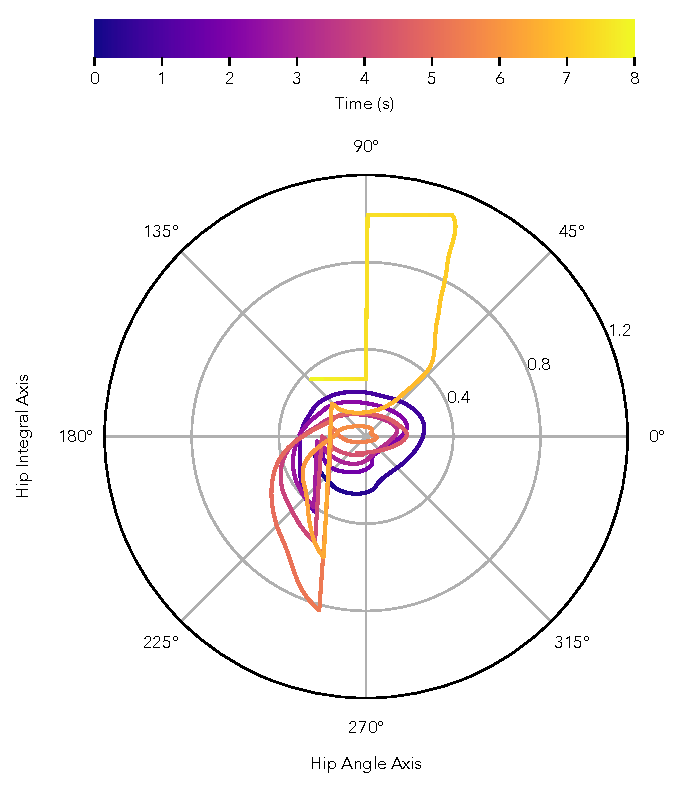
\includegraphics[width=\textwidth]{phase_var_plot_vs_polar}
    \caption[Phase angle over eight seconds of walking.]{Phase angle over eight
    seconds of walking. Drift in the integral term caused irregularities in the
    phase angle plot.}\label{fig:phase_var_polar}
\end{figure}
\Cref{fig:phase_var_polar} shows an example phase portrait from an eight second
walking bout. From this figure, we see that towards the latter end of the trial,
the integral term tends to drift towards the end of stance before being reset to
zero at heel strike. These irregularities step from the sensitivity of the
integral term to the hip angle trajectory and cause the phase angle to trace
form a nonlinear curve in time.

Therefore, to prevent excessively unnatural phase trajectories, we also
implemented time based upper and lower bounding of the phase. In this scheme,
the normalized phase,
\begin{align}
    \bar \upsilon(t) = \frac{\upsilon(t) - \upsilon(0)}{2 \pi}
\end{align}
is lower and upper bound by third order polynomial functions of time. The lower
bound polynomial intersects three points: $\phi(t=0) = 0$,
$\phi(t=\nicefrac{T}{2}) = \nicefrac{1}{4}$ and $\phi(t = T) = 1$ while the
upper bound polynomial intersects: $\phi(t=0) = 0$,
$\phi(t=\nicefrac{T}{2}) = \nicefrac{3}{4}$ and $\phi(t = T) = 1$. The stride
duration $T$ was estimated as the median of the last five steps. Finally, the
constrained phase variable estimate was low pass filtered by a $2^\tn{nd}$ order
Butterworth filter with a cut off frequency of \unit[10]{Hz}.

The phase estimate was used to look up the desired knee and ankle angles. PID
control was then used to calculate the desired torque for the actuators which
was then achieved by the low level torque control (\cref{sec:sea_control}).

\begin{figure*}[t]
    \centering 
    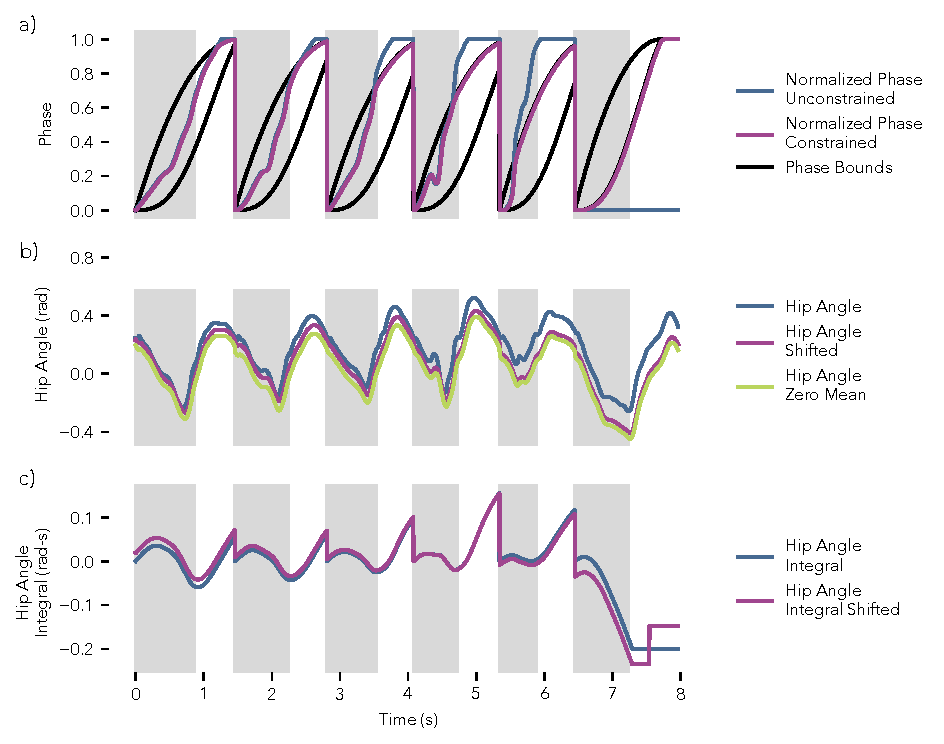
\includegraphics[width=\textwidth]{phase_var_plot_vs_time}
    \caption[Results from test of unified phase variable controller.]{Results
    from test of unified phase variable controller. Step to step variability
    causes significant divergence in the integral term, leading to an unstable
    phase estimate.}\label{fig:phase_var_vs_time}
\end{figure*}
Row 1 of \cref{fig:phase_var_vs_time} shows the unconstrained and constrained
phase estimates in blue and purple respectively and the lower and upper bounds
in black. The phase estimate only remained within the bounds for the first step.
After that, the phase estimate needed to be constrained by the upper bound
earlier and earlier in each step.

The hip angle plot in the second row, shows there is significant variability in
the hip angle trajectory from step to step. Consequently, the hip angle integral
(row 3) does not reach zero at the beginning of each stance (stance phase
designated by grey shaded regions). The drift in the integral term occurs
despite updates to the shifted hip angle (purple row 2) and zero-mean hip angle
(green row 2). 

The resultant control action on the prosthesis, seemed to drive a positive
feedback loop wherein increased phase angle in late stance drives knee flexion
and ankle push off leading into swing. Increased knee flexion torque and ankle
plantarflexion also flex the hip more, which further drives the phase estimate
forward. Consequently, the gait was driven faster and faster, as shown by
decreasing duration of stance (grey shaded regions). Also, a potential
contributor to this positive feedback loop was an over-reliance on integral
action in the ankle, which is slow to build up the required plantarflexion
torque; a feedforward torque term might be helpful for generating torque as a
function of phase. The changing duration of stance also caused variation in hip
integral leading to more gait instability. Due to these issues, we were not able
to achieve hands free-walking for any duration of time, and only managed walking
with hand rail support for a few seconds at a time.

While these problems could be rectified with tighter bounds on the phase, this
would make the controller closer to a time-based strategy, which would make
volitional control impossible. Therefore, in the following sections we propose
using a more established method of state estimation, an extended Kalman filter,
to estimate the phase during gait. Using a Kalman allows us to specify dynamics
for the phase, which help keep its trajectory smooth. Furthermore, it allows us
to incorporate information from more than two sources, while considering the
intrinsic variation of each signal.
